\chapter{Riemann Pump circuit design}
\label{ch:design}
% \textit{Description of the approach you have taken to solve the scientific or technical problem which you were posed. Outline the design, the methodology and overall structure of your experimental approach}\\
The goal was to design an arbitrary waveform generator for a signal bandwidth of \SI{6}{\giga \hertz}.
For the implementation in a base station, the most promising technology was \gls{ab:gan}.
\gls{ab:gan} \glspl{ab:hemt} were used for the high speed switches, which served as a voltage controlled current source.
Based on the chosen technology a suitable push-pull concept were found \cite{MaksimovicPaper} to show the feasibility of the concept.
The attention was rather drawn to proof the concept than to optimize for energy consumption or efficiency.
In the design process a suitable load impedance and the right dimension of the used components were found.

\section{Approach and implementation of the Riemann Pump}
As stated in chapter \ref{IdeaRiemannPump} the circuit needed high speed switches, which were capable to drive power.
The absence of a p-type transistor in \gls{ab:gan} technology made it challenging to find a suitable concept to realize the push-pull stage.
Since the n-type \glspl{ab:hemt} needed a negative gate source voltage \gls{sy:vgs}, the high side switch could not be implemented without a driver circuit.
The source contact of the high side switch, realized by a n-type \gls{ab:gan} \gls{ab:hemt}, was connected to the output of the test circuit.
Since the potential at the output was not constant, this high side switch needed a driver circuit.
A suitable driver circuit was found in \cite{MaksimovicPaper}, where the principle of a push-pull stage for power applications is described.\\
One possible approach to design a Riemann Pump is shown in Fig. \ref{fig:SchematicRiemannPump}.

\begin{figure}[ht]
	\centering
  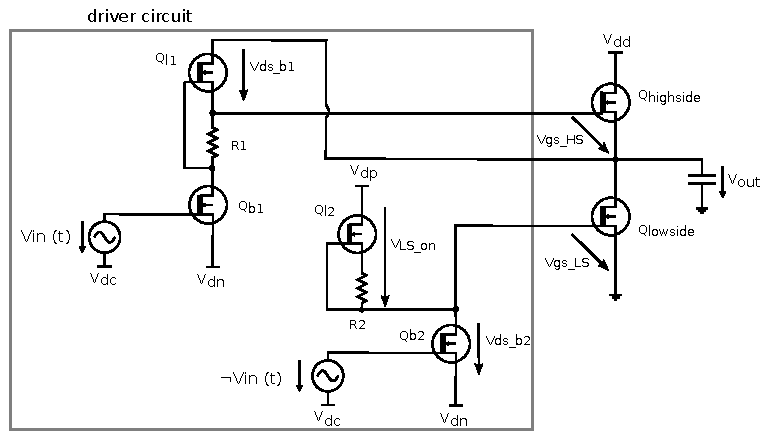
\includegraphics{Schematic_RP_concept2.pdf}
	\caption{Schematic of a push-pull stage with corresponding driver circuit}
	\label{fig:SchematicRiemannPump}
\end{figure}

The benefit of the integrated driver circuit was the improved efficiency of switching.
The transistor switching speed was determined by the dimension of the driver circuit.
If the switching speed was increased, the gate driving current \gls{sy:IG} has to be increased to switch the transistors.
 
\section{Identification of the load impedance}
The signal is generated at the input stage of a linear power amplifier, as described in \ref{ch:fundamentals}.
This input stage is modelled with a \gls{ab:gan} \gls{ab:hemt} with a gate length of \SI{0.25}{\micro \meter}.
Considering a \SI{20}{\watt} power amplifier for transmission purposes, led to a \gls{ab:gan} \gls{ab:hemt} with a total gate periphery of \SI{4}{\milli \metre}, based on an approximation for the power density of \SI[per-mode=fraction]{5}{\watt\per\milli\metre} gate periphery  \cite{Maroldt2010}, \cite{GaNBook}.
Simulations confirmed this approximation as an output power density of \SI[per-mode=fraction]{5.6}{\watt\per\milli\metre} at $V_{DS} = 25 V$ was measured.
The simulated power amplifier is biased with respect to the maximum \gls{ab:mag}, which led to a bias of $V_{GS} = -1.5 V$ at $V_{DS} = 25 V$.
After the determination of the bias point, a S-parameter simulation yielded the input reactance of the power amplifier as seen in Figure \ref{fig:inputReactance}.

\begin{figure}[ht]
	\centering
  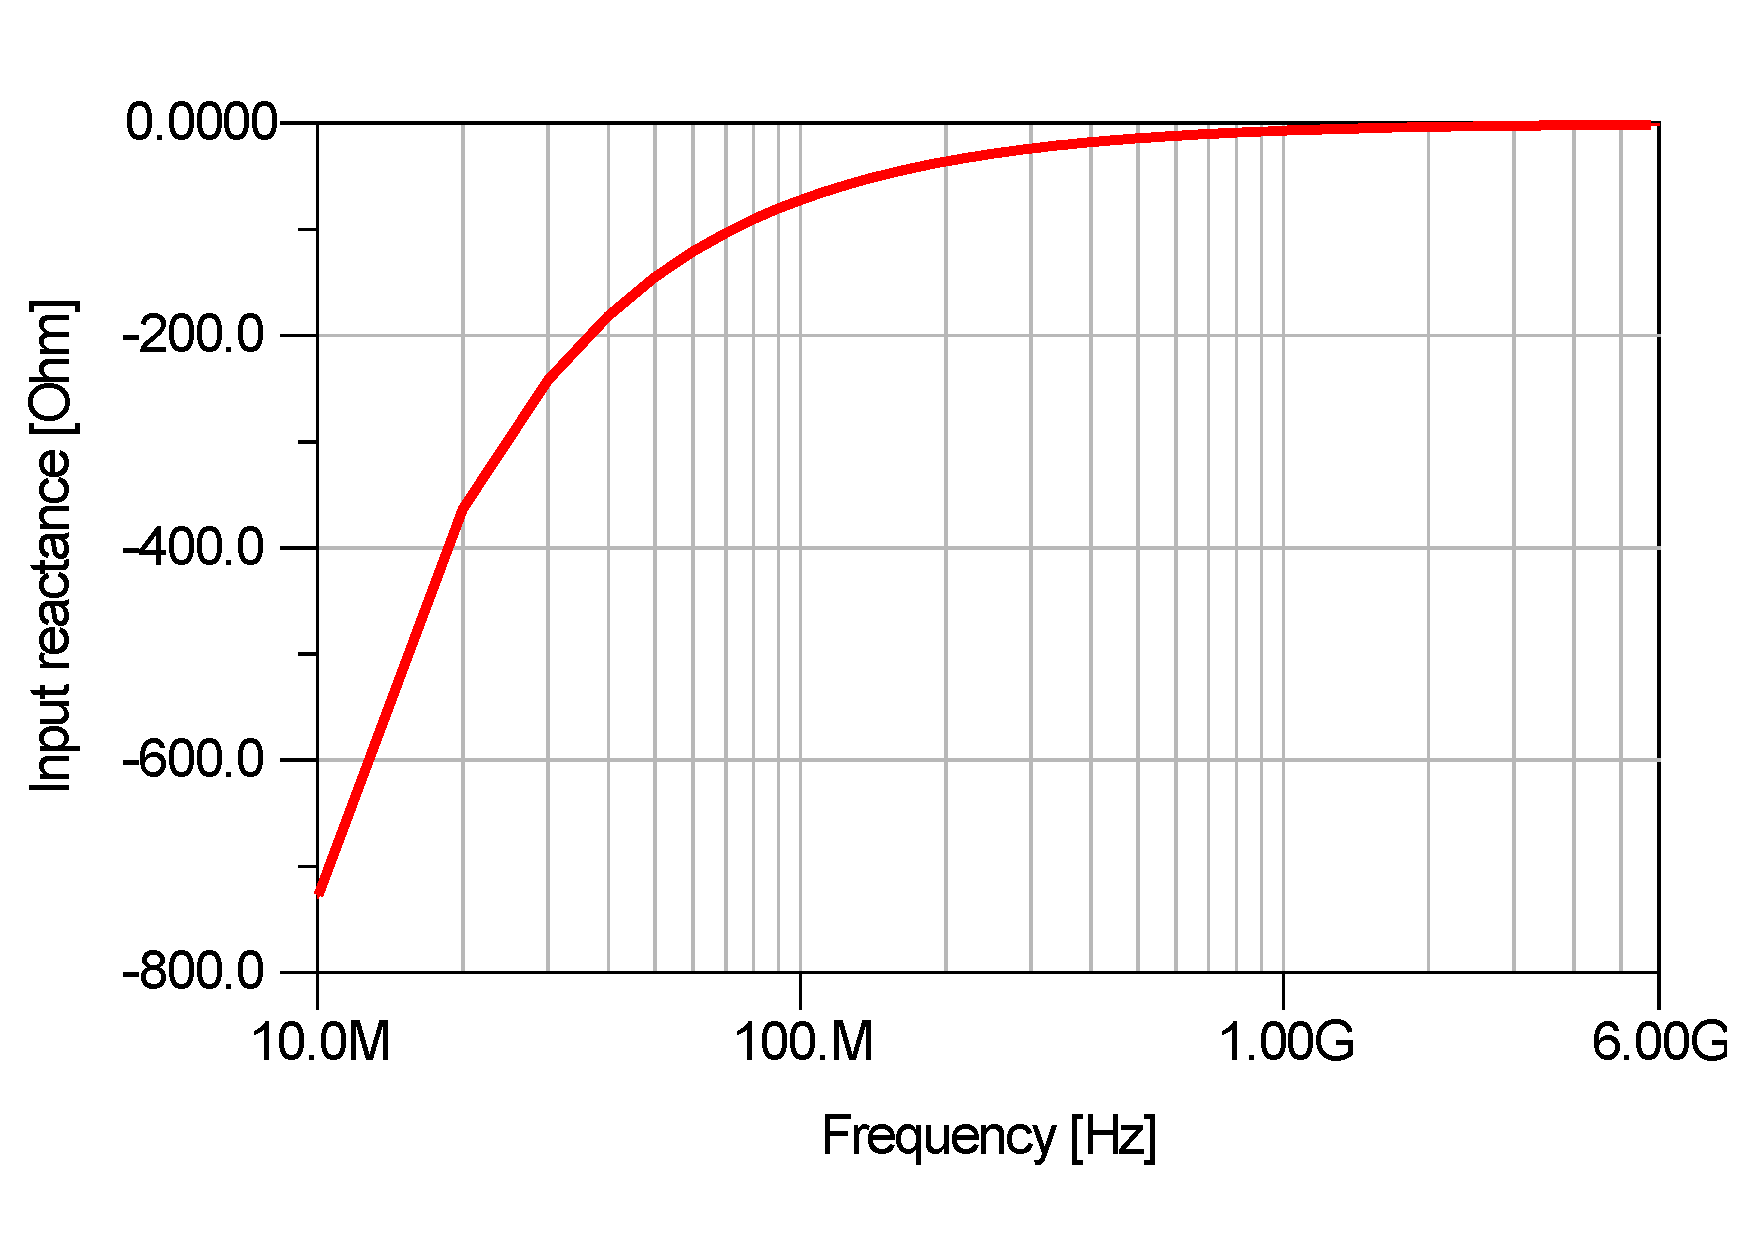
\includegraphics[width=1\textwidth]{inputReactance.pdf}
	\caption{load reactance}
	\label{fig:inputReactance}
\end{figure}

Since only the capacitive behaviour of the load impedance is of interest, the real part is neglected.
Figure \ref{fig:inputReactance} shows the input reactance over the frequency range from \SI{10}{\mega \hertz} to \SI{6}{\giga \hertz} in a logarithmic scale.
As the reactance of the simulated power amplifier is nearly constant for the frequency of \SI{1}{\giga \hertz} and beyond, this led to the assumption that (dispersion)parasitic effects came into play.
The input reactance $X_c$ is defined as

\begin{equation}
	X_c = -\frac{1}{\omega C},
\end{equation}
\label{eq:reactance}
and is plotted in Figure \ref{fig:inputReactance}.

Solving for the capacitance yielded:
\begin{equation}
	C = \frac{-1}{\omega X_c},
\end{equation}

Figure \ref{fig:inputCap_log} shows the effect of decreasing capacitance with frequency.

\begin{figure}[ht]
	\centering
  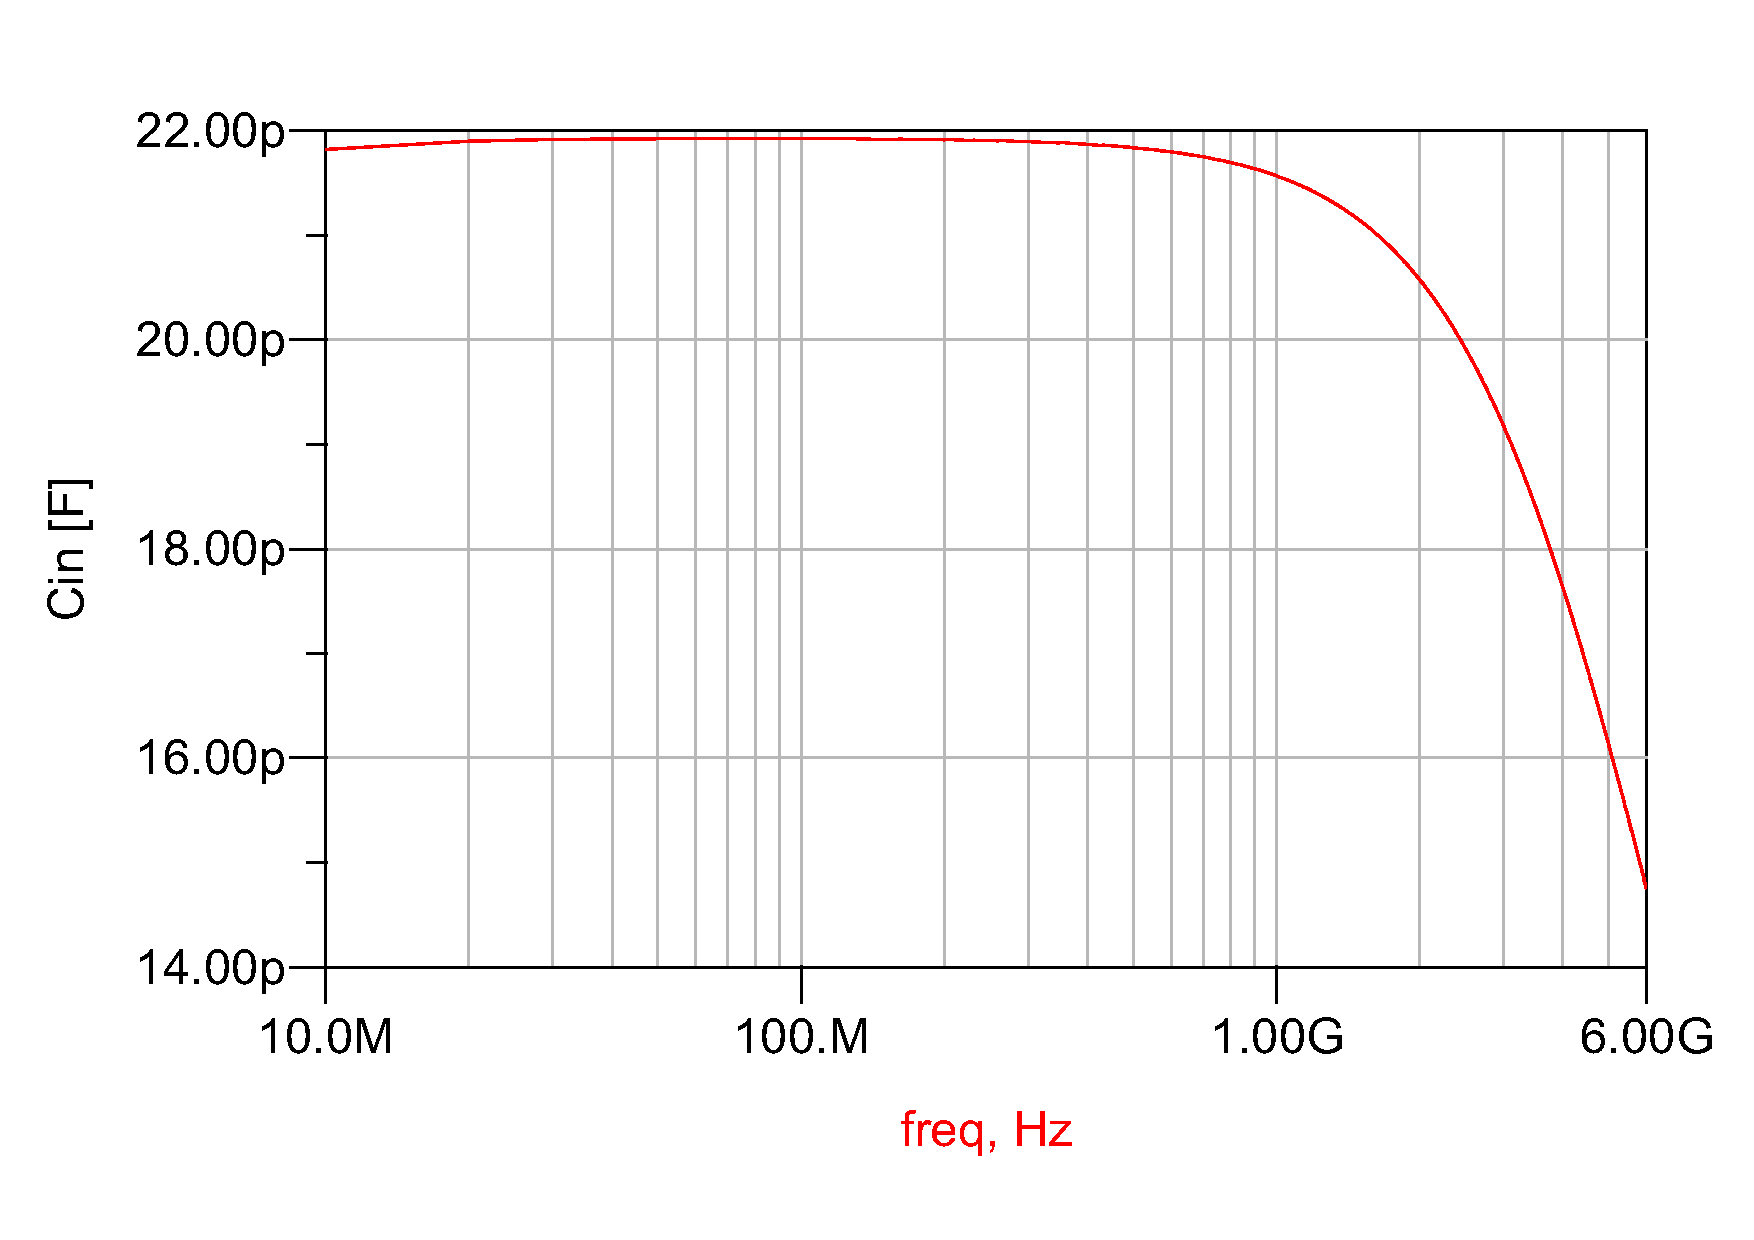
\includegraphics[width=1\textwidth]{inputCap_log.pdf}
	\caption{load capacitance log}
	\label{fig:inputCap_log}
\end{figure}

The value of the input capacitance stays constant for frequencies below \SI{1}{\giga \hertz} which was assumed. 
For the \gls{ab:rf} range the capacitance drops.

An increase of the input impedance was expected, but an increase of the input capacitive was not [\textbf{REFERENCE}](parasitic effects).

Due to the non-linearity of the transistor model \cite{vitanovnon}, the input impedance of the power stage is simulated.

The frequency dependent input impedance [\textbf{REFERENCE}], which corresponds to the load impedance of the designed Riemann pump circuit, is determined by S-parameter simulations.

This transistor model \gls{ab:hemt} (IAF\_GE\_MSL\_ A204/IAF\_GaN25\_HEMT\_CS\_LS\_SHfull) used in \gls{ab:ads} were modelled at the \gls{ab:iaf}\cite{model} and is based on a state-space approach.\\ 
For simulation purposes four transistors were modelled in parallel, each with 8 finger and \SI{125}{\micro \metre} gate width to reach the required gate periphery.
The bias point was determined with the \gls{ab:mag}, to be $V_{GS} = -1.5 V$, $V_{DS} = 15 V$.
This led to an impedance shown in Figure [\textbf{INSERT COMPLEX IMPEDANCE}].

%\begin{equation}
%Z = R - jX_c
%\end{equation}

% small signal is not considered, since only the curent integration is important
%With the help of the $S_{11}$ parameter plotted in the smith chart Fig. \ref{fig:smith_load_impedance} the load impedance can be determined.
%The load impedance got a capacitive reactance.
% The real part of the impedance is roughly $R = \SI{1.89}{\ohm}$, while the imaginary part is capacitive.
An important point is the input capacitance is increasing with frequency. 
While it is normal that the imaginary part of the impedance is increasing with frequency, the input capacitance is not.

 \begin{figure}[ht]
	\centering
  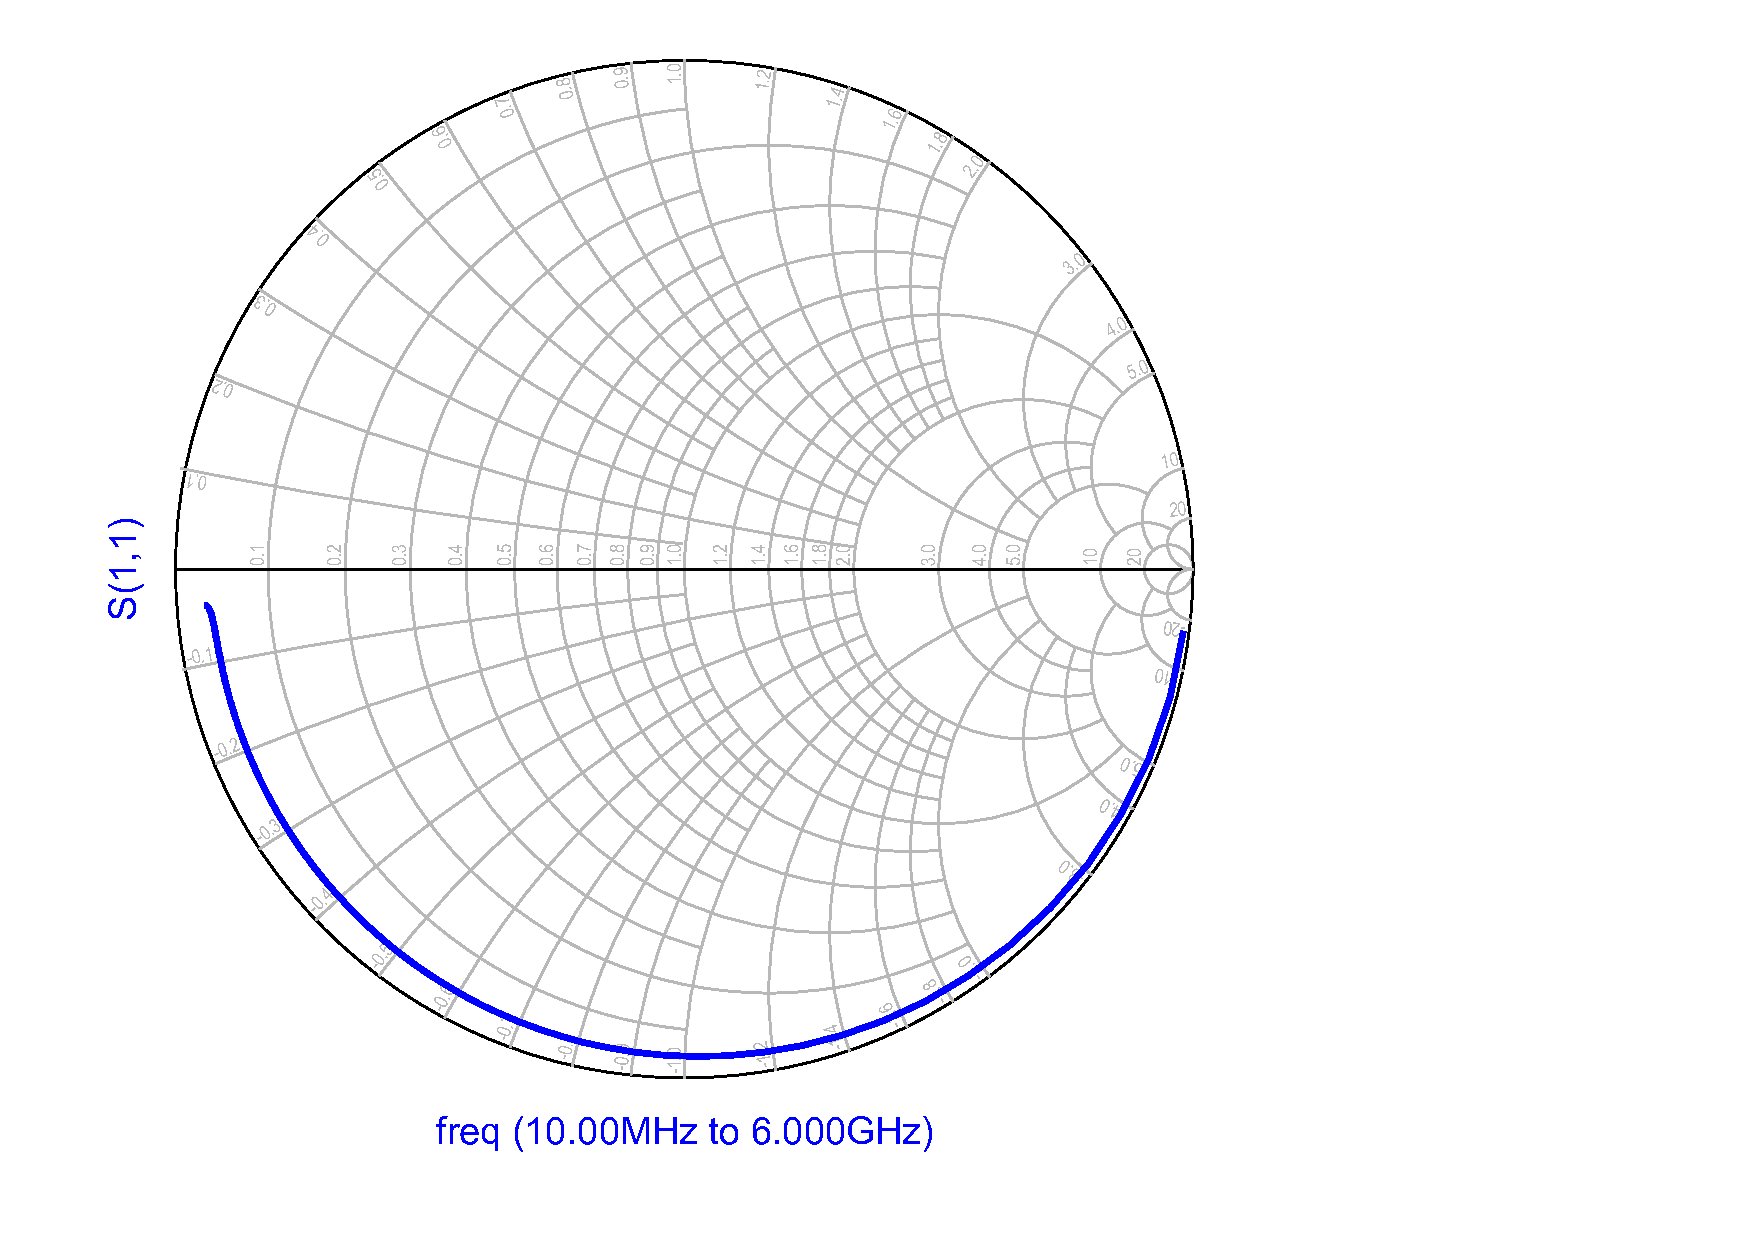
\includegraphics[draft,width=1\textwidth]{S_param_LoadImpedance.pdf}
	\caption{smith chart representing the load impedance}
	\label{fig:smith_load_impedance}
\end{figure}

The load capacitance is calculated through the complex impedance:
\begin{equation}
C = \frac{1}{2 \pi f X_c}
\end{equation}

 \begin{figure}[ht]
	\centering
  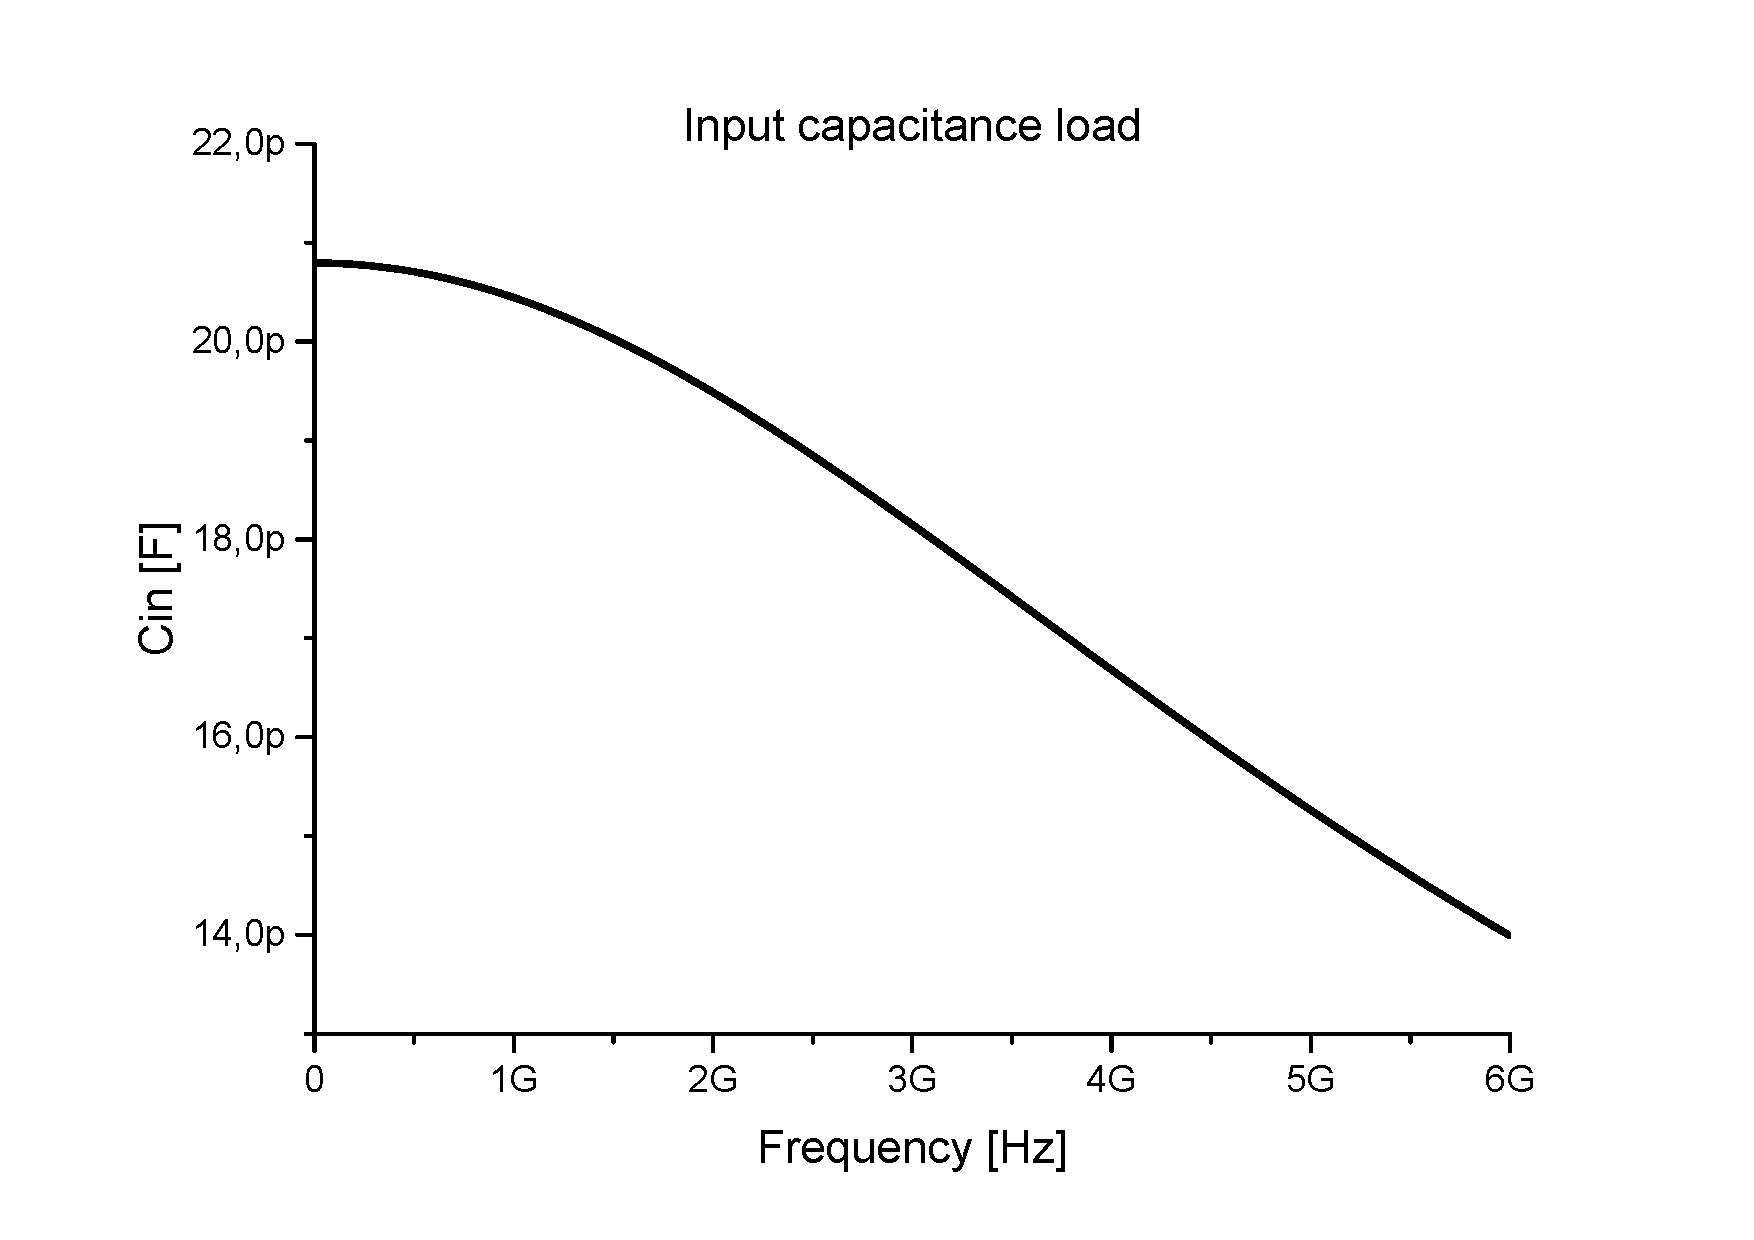
\includegraphics[draft,width=0.75\textwidth]{InputCap_LoadImpedance_6GHz.pdf}
	\caption{frequency dependent input capacitance of the load - log scale}
	\label{fig:smith_load_impedance_inC}
\end{figure}

\section{Dimension of the used components}
The transistor dimension were... Different for driver circuit and power circuit... resistor to reduce the energy  consumption, for higher efficiency.
The approach of the push-pull stage Maksimovic, Maroldt.
Approach of theoretical and synthesized signal -> MatLab generation of Riemanncode, SNR.\\ Stability, driver concept, energy consumption, frequency bandwidth, gain
Schematic design in Advanced Design System 2014. concept, ideas... 
Control voltage of 5 V realization with OPAMPS? Possible to overdrive opamps instead of using broadband ppa. 

\section{Circuit design summary}
The speed of the switches is crucial as a broadband signal should be synthesized.
Using a well known concept got the advantage of verification, validation and knowing the drawbacks.
In addition to this it was possible to use the work of a former employee, which makes it easier to realize, since a new MMIC desing was not in the scope of this thesis.\\
\textit{Drawbacks, problems, challenges.}
Same realisation problems and difficulties: Problem of BANDWIDTH, Vpp of control signal (5V pp for GaN transistors), high side driver, no complementary transistors available in III-V technology, low loss driver, high speed driver, digital control driver, too high energy consumption (stability???)
\textbf{bandwidth limitation}
\textit{The lower bound is determined by the sampling time (inverse of the sampling frequency) and the smallest current achieved with the dimensioned transistors.
 The smallest achievable current times the smallest sampling time (highest sampling frequency) determine the smallest absolute slope achievable. \\
% \textbf{Is every signal possible to create? a rect signal has too steep flanks to create. The signal bandwidth ranges from DC to 6 GHz but what is the amplitude range? Is there a limitation regarding the amplitude?}
\\
The smallest current is determined by the dimension of the transistor, which drives into saturation. 
The smallest saturated current is determined by the push-pull transistor geometry, here: 532 mA.}
The dimension of the switching transistors, which represent a voltage controlled current source, determines the maximum current flowing.
This current source is controlled by a digital signal which determines it to be fully open or to be closed, as a switch.
Therefore the current is not controlled by the transistor itself, it flows at its maximum or it does not flow anyway.
This dimension determines the slope of the resulting voltage steps.
A small transistor dimension could synthesize signals to a very low signal frequency while a bigger one would fully charge the output capacitor which will clip the output signal.

If the transistor dimension is chosen to be bigger, the higher signal frequency could be synthesized with a decent voltage swing but the low signal frequencies would turn into a rectangular shape. 

In contrast to the small one a bigger one will be able to synthesize a signal at 6GHz due to the fact that the amplitude would be moderate.
This is one problem which restrict the signal bandwidth to a smaller one than the \gls{ab:dc} to \SI{6}{\GHz}.